\chapter{Numerical experiments}

% In this section the results of numerical experiments should be placed.
% They can confirm or contradict the expectation from the previous sections. 
% The forms of result presentation are plots, tables, histograms, pictures, etc.
% \begin{enumerate}
%     \item Enumerating languages and programs used in the research.
%     \item Describing in detail data sets you used.
%     \item Presenting the metrics used.
%     \item Presenting the results achieved in the experiment.
%     \item Comparing the results of the experiment with those obtained using other methods.
%     \item Outlining the benefits of the used method.
% \end{enumerate}
\section{Implementation Details}  
The experiments were implemented in \texttt{Python 3.9} using the following libraries:  
\begin{itemize}  
    \item \texttt{PyTorch} and \texttt{Torchvision} for model construction and training,  
    \item \texttt{Dicom2img} and \texttt{Tifffile} for CT scan preprocessing,  
    \item \texttt{Tensorboard} and \texttt{Matplotlib} for metrics logging and visualization.  
\end{itemize}  

\section{Dataset}  
The dataset comprised 29 high-resolution 3D CT scans of crocodilian skulls, divided into:  
\begin{itemize}  
    \item \textbf{Training}: 24 scans (6,012 2D slices),  
    \item \textbf{Validation}: 5 scans (1,365 2D slices).  
\end{itemize}  
Each 2D slice was resized to \(256 \times 256\) pixels and augmented with the following transformations: random horizontal flip, random vertical flip and random rotation (from -60 to +60 degrees)

\section{Metrics and Training Protocol}  
The U-Net model was trained for 480 epochs using:  
\begin{itemize}  
    \item \textbf{Loss Function}: \(\mathcal{L} = \text{DiceLoss} + \text{BCELoss}\),  
    \item \textbf{Optimizer}: AdamW (\(lr = 1 \times 10^{-5}\)),  
    \item \textbf{Scheduler}: CosineAnnealingLR (\(T_{\text{max}} = 10\), \(\eta_{\text{min}} = 0\)).  
\end{itemize}  
Performance was evaluated using:  
\begin{itemize}  
    \item \textbf{Dice Coefficient}: Measures segmentation overlap,  
    \item \textbf{Precision}: \(\frac{\text{True Positives}}{\text{True Positives} + \text{False Positives}}\),  
    \item \textbf{Recall}: \(\frac{\text{True Positives}}{\text{True Positives} + \text{False Negatives}}\).  
\end{itemize}  

\section{Results}  
Training and validation metrics are summarized in Table~\ref{tab:metrics}, with loss curves shown in Figure~\ref{fig:loss}, metrics curves in Figure~\ref{fig::Dice}, Figure~\ref{fig::Precision}, Figure~\ref{fig::Recall} and example results in Figure~\ref{fig::Prediction1}.  
\begin{table}[ht]  
    \centering  
    \caption{Segmentation performance on training and validation sets.}  
    \label{tab:metrics}  
    \begin{tabular}{lccc}  
        \toprule  
        \textbf{Set} & \textbf{Dice} & \textbf{Precision} & \textbf{Recall} \\  
        \midrule  
        Training & 0.81 & 0.83 & 0.81 \\  
        Validation & 0.75 & 0.79 & 0.78 \\  
        \bottomrule  
    \end{tabular}  
\end{table}  

\begin{figure}[ht]  
    \centering  
    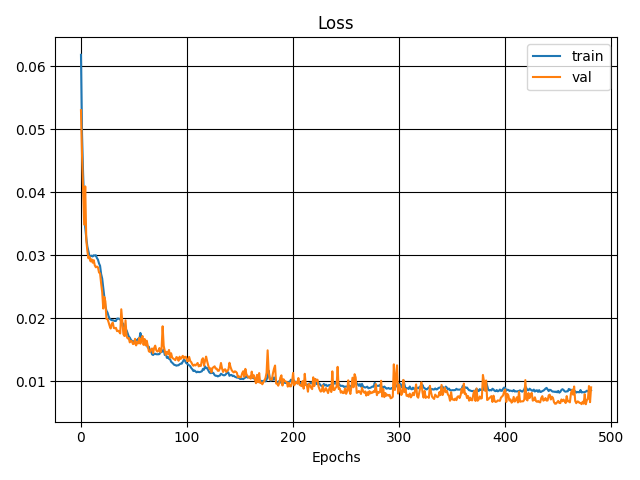
\includegraphics[width=0.9\textwidth]{images/plots/Loss.png}
    \caption{Training and validation loss curves. The model converges stably with minimal overfitting.}  
    \label{fig:loss}  
\end{figure}  


\section{Benefits of the Proposed Method}  
\begin{itemize}  
    \item \textbf{Reproducibility}: Eliminates observer bias inherent in manual segmentation.  
    \item \textbf{Scalability}: Processes 3D scans as 2D slices, reducing GPU memory demands.  
    \item \textbf{Robustness}: Augmentation strategies improved generalization to low-contrast regions.  
\end{itemize}  


\begin{figure}[!htb]
    \centering
    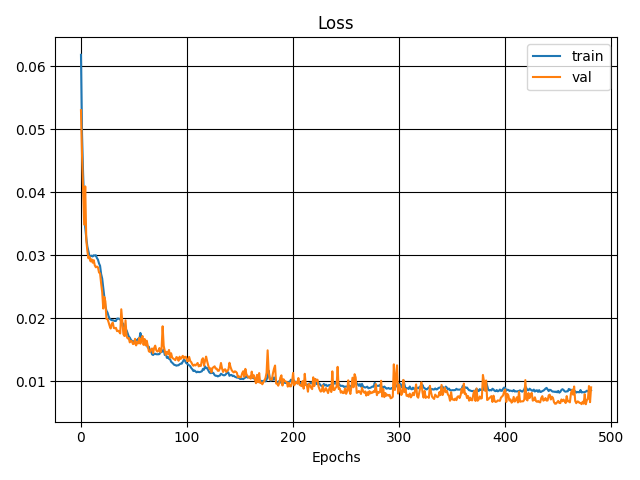
\includegraphics[width=0.9\textwidth]{images/plots/Loss.png}
    \caption{Loss during training}
    \label{fig::loss}
\end{figure}

\begin{figure}[!htb]
    \centering
    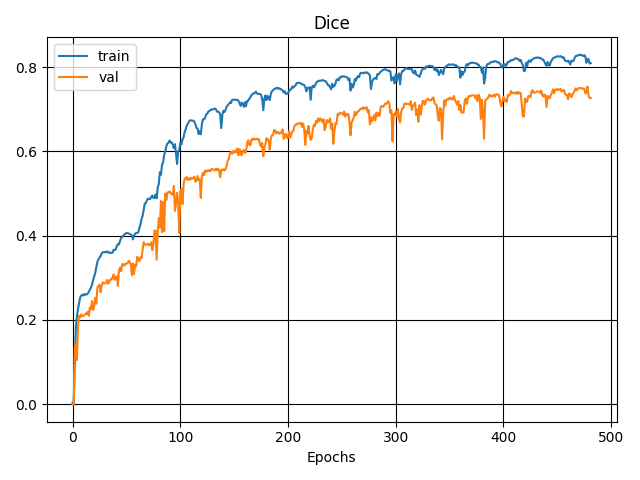
\includegraphics[width=0.9\textwidth]{images/plots/Dice.png}
    \caption{Dice score during training}
    \label{fig::Dice}
\end{figure}



\begin{figure}[!htb]
    \centering
    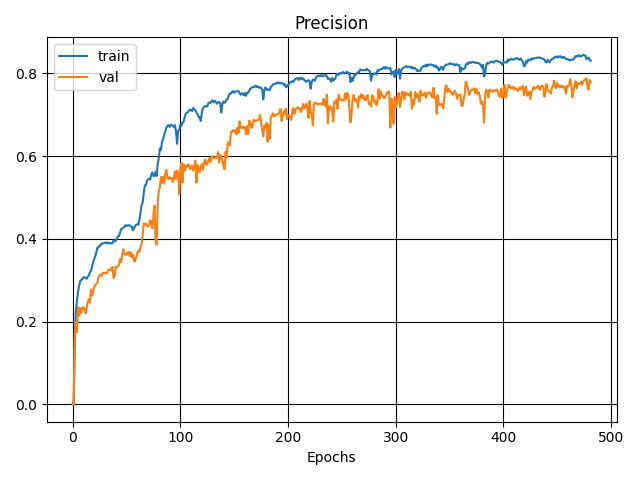
\includegraphics[width=0.9\textwidth]{images/plots/Precision.png}
    \caption{Precision during training}
    \label{fig::Precision}
\end{figure}

\begin{figure}[!htb]
    \centering
    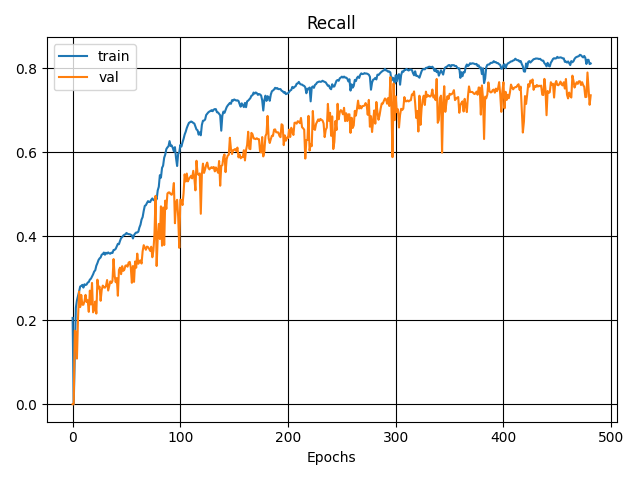
\includegraphics[width=0.9\textwidth]{images/plots/Recall.png}
    \caption{Recall during training}
    \label{fig::Recall}
\end{figure}

\begin{figure}[!htb]
    \centering
    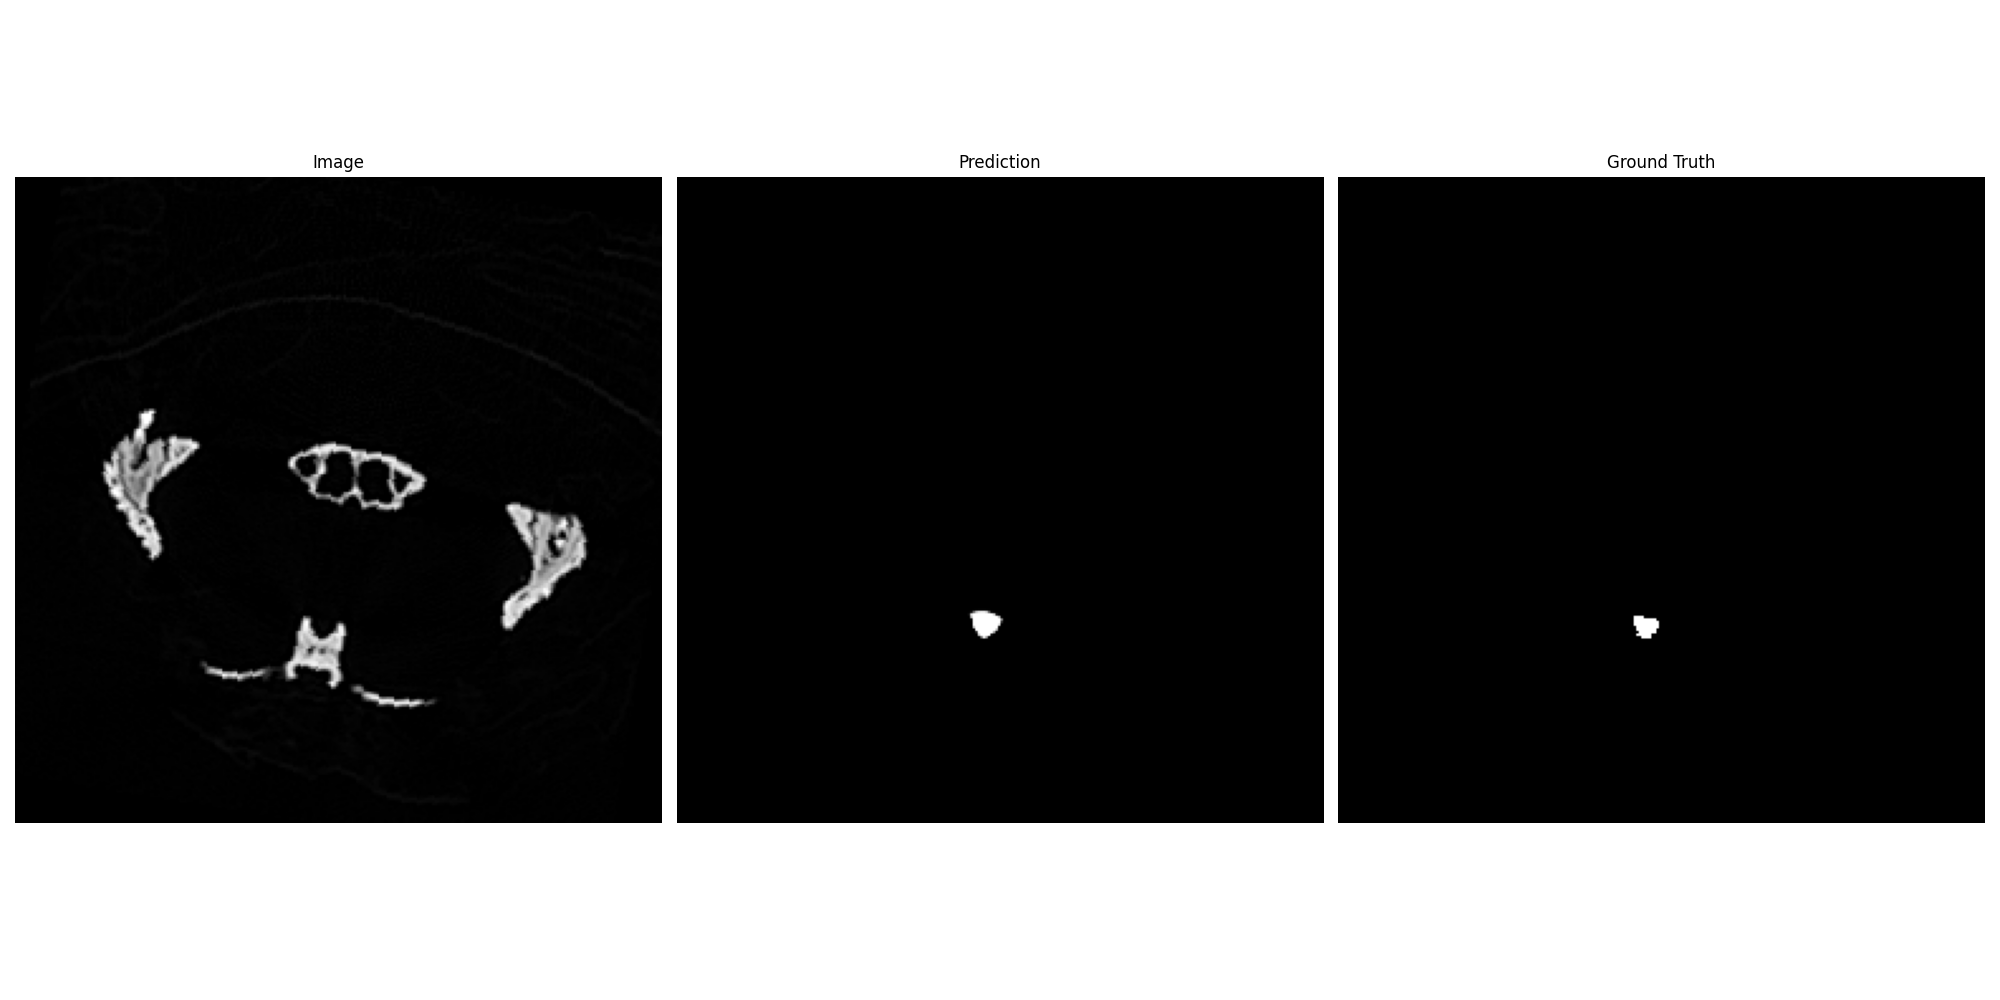
\includegraphics[width=0.99\textwidth]{images/results/prediction1.png}
    \caption{Example of prediction}
    \label{fig::Prediction1}
\end{figure}